\documentclass[11pt]{article}
\usepackage{amsmath,amssymb,amsthm}
\usepackage{tikz}
\usetikzlibrary{positioning,calc}
\usepackage{booktabs}
\usepackage{enumitem}

\newtheorem{theorem}{Theorem}[section]
\newtheorem{lemma}[theorem]{Lemma}
\newtheorem{proposition}[theorem]{Proposition}
\newtheorem{corollary}[theorem]{Corollary}
\theoremstyle{definition}
\newtheorem{definition}[theorem]{Definition}
\newtheorem{example}[theorem]{Example}
\theoremstyle{remark}
\newtheorem{remark}[theorem]{Remark}

\newcommand{\ZZ}{\mathbb{Z}}
\newcommand{\NN}{\mathbb{N}}
\newcommand{\Gray}{\mathsf{G}}
\newcommand{\entry}{\mathsf{entry}}
\newcommand{\exits}{\mathsf{exit}}

\title{Hilbert Curves via Oriented Gray Codes}
\author{}
\date{}

\begin{document}
\maketitle

\begin{abstract}
We present a framework for Hilbert curves based on Gray codes and orientations.
The key insight is that a Hilbert curve is a hierarchy of \emph{oriented Gray codes},
and the continuity of the curve follows from a single observation:
orientation transformations preserve adjacency.
This framework extends naturally to anisotropic boxes (unequal side lengths)
via an embedding operation that preserves the gluing conditions.
\end{abstract}

%=============================================================================
\section{Gray Codes on the Hypercube}
%=============================================================================

We begin with the hypercube and the notion of adjacency.

\begin{definition}[$n$-cube]
The \emph{$n$-cube} is the set $\{0,1\}^n$ of binary strings of length $n$.
We call its elements \emph{corners} or \emph{vertices}.
\end{definition}

\begin{definition}[Adjacency]
Two corners $u, v \in \{0,1\}^n$ are \emph{adjacent} if they differ in exactly one coordinate.
Equivalently, $u \oplus v = \mathbf{e}_a$ for some axis $a \in \{0, \ldots, n-1\}$,
where $\mathbf{e}_a$ is the standard basis vector with a 1 in position $a$ and 0s elsewhere,
and $\oplus$ denotes XOR (coordinatewise addition mod 2).
\end{definition}

\begin{definition}[Gray code]
A \emph{Gray code} on $\{0,1\}^n$ is a sequence $(c_0, c_1, \ldots, c_{2^n-1})$
that visits each corner exactly once, with consecutive corners adjacent.
\end{definition}

In other words, a Gray code is a Hamiltonian path on the hypercube graph.

\begin{example}[The standard Gray code for $n = 2$]\label{ex:gray2d}
The binary reflected Gray code $\Gray: \{0,1,2,3\} \to \{0,1\}^2$ is:
\[
\Gray(0) = 00, \quad
\Gray(1) = 01, \quad
\Gray(2) = 11, \quad
\Gray(3) = 10.
\]
Consecutive values differ in one bit:
$00 \to 01$ (bit 0),
$01 \to 11$ (bit 1),
$11 \to 10$ (bit 0).
\end{example}

\begin{example}[The standard Gray code for $n = 3$]\label{ex:gray3d}
\[
\begin{array}{c|c}
i & \Gray(i) \\
\hline
0 & 000 \\
1 & 001 \\
2 & 011 \\
3 & 010 \\
4 & 110 \\
5 & 111 \\
6 & 101 \\
7 & 100 \\
\end{array}
\]
The sequence visits all 8 corners of the 3-cube, changing one bit at each step.
\end{example}

The standard binary reflected Gray code $\Gray: \{0, \ldots, 2^n - 1\} \to \{0,1\}^n$
is defined by $\Gray(i) = i \oplus \lfloor i/2 \rfloor$ (interpreting integers as bit vectors).
The key property we need is:

\begin{proposition}[Gray code adjacency]
For all $i \in \{0, \ldots, 2^n - 2\}$, the corners $\Gray(i)$ and $\Gray(i+1)$ are adjacent.
\end{proposition}

This is the standard property of Gray codes and is well-known.

%=============================================================================
\section{Orientations}
%=============================================================================

A single Gray code gives us one Hamiltonian path through the cube.
To build Hilbert curves, we need to place \emph{differently oriented} copies
of this path in different subcubes. We now formalize what ``orientation'' means.

\begin{definition}[Axis permutation action]
Let $\pi \in \mathrm{Sym}(n)$ be a permutation of $\{0, \ldots, n-1\}$.
We define the action of $\pi$ on a corner $v \in \{0,1\}^n$ by permuting coordinates:
\[
(\pi \cdot v)_a := v_{\pi^{-1}(a)}.
\]
In words: the value at position $a$ in the output comes from position $\pi^{-1}(a)$ in the input.
\end{definition}

\begin{remark}
We use $\pi^{-1}$ so that this is a left action: $(\pi_1 \circ \pi_2) \cdot v = \pi_1 \cdot (\pi_2 \cdot v)$.
\end{remark}

\begin{definition}[Orientation]
An \emph{orientation} on the $n$-cube is a pair $(e, \pi)$ where:
\begin{itemize}[nosep]
\item $e \in \{0,1\}^n$ is the \emph{entry corner}, and
\item $\pi \in \mathrm{Sym}(n)$ is an \emph{axis permutation}.
\end{itemize}
\end{definition}

\begin{definition}[Oriented Gray code]
Given an orientation $(e, \pi)$, the \emph{oriented Gray code} is the sequence:
\[
c_i := \pi \cdot \Gray(i) \oplus e, \qquad i = 0, \ldots, 2^n - 1.
\]
\end{definition}

The oriented Gray code starts at corner $e$ (since $\Gray(0) = 0\cdots0$, so $c_0 = e$),
and the axis permutation $\pi$ rotates/reflects the ``shape'' of the path.

\begin{lemma}[Orientation preserves adjacency]\label{lem:orient-adj}
If $(c_0, \ldots, c_{2^n-1})$ is a Gray code, then for any orientation $(e, \pi)$,
the sequence $(\pi \cdot c_0 \oplus e, \ldots, \pi \cdot c_{2^n-1} \oplus e)$ is also a Gray code.
\end{lemma}

\begin{proof}
Suppose $c_i$ and $c_{i+1}$ differ in exactly bit $a$, i.e., $c_i \oplus c_{i+1} = \mathbf{e}_a$.

First, XOR with $e$ does not change differences:
$(c_i \oplus e) \oplus (c_{i+1} \oplus e) = c_i \oplus c_{i+1} = \mathbf{e}_a$.

Second, the permutation $\pi$ moves the differing bit to position $\pi(a)$:
$(\pi \cdot c_i) \oplus (\pi \cdot c_{i+1}) = \pi \cdot (c_i \oplus c_{i+1}) = \pi \cdot \mathbf{e}_a = \mathbf{e}_{\pi(a)}$.

So consecutive corners in the oriented sequence still differ in exactly one bit.
\end{proof}

\begin{example}[Orientations on the 2-cube]\label{ex:orient2d}
Consider the standard 2D Gray code from Example~\ref{ex:gray2d}, drawn as a path:
\[
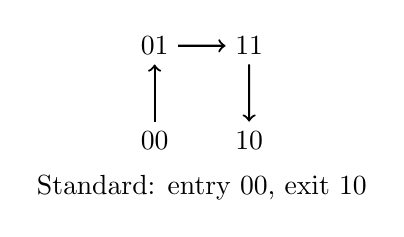
\begin{tikzpicture}[scale=1.2, baseline=(current bounding box.center)]
\node (00) at (0,0) {$00$};
\node (01) at (0,1) {$01$};
\node (11) at (1,1) {$11$};
\node (10) at (1,0) {$10$};
\draw[thick,->] (00) -- (01);
\draw[thick,->] (01) -- (11);
\draw[thick,->] (11) -- (10);
\node at (0.5,-0.5) {Standard: entry $00$, exit $10$};
\end{tikzpicture}
\]

With orientation $(e, \pi) = (10, \text{swap})$ where $\pi$ swaps axes 0 and 1:
\[
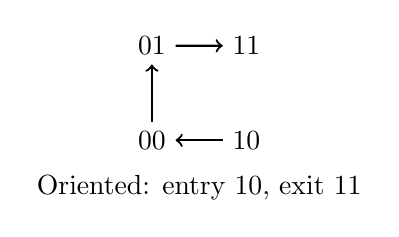
\begin{tikzpicture}[scale=1.2, baseline=(current bounding box.center)]
\node (00) at (0,0) {$00$};
\node (01) at (0,1) {$01$};
\node (11) at (1,1) {$11$};
\node (10) at (1,0) {$10$};
\draw[thick,->] (10) -- (00);
\draw[thick,->] (00) -- (01);
\draw[thick,->] (01) -- (11);
\node at (0.5,-0.5) {Oriented: entry $10$, exit $11$};
\end{tikzpicture}
\]
The path still visits all four corners with unit steps, just starting and ending differently.
\end{example}

%=============================================================================
\section{The Generator and Gluing}
%=============================================================================

A Hilbert curve is built by recursively subdividing a cube into $2^n$ subcubes
and placing an oriented copy of the curve in each. The \emph{generator} specifies
how each child's orientation relates to its parent.

\begin{definition}[Generator]
A \emph{generator} is a function $\mu: \{0, \ldots, 2^n - 1\} \to \text{Orientations}$
that maps each child index $w$ to a relative orientation $\mu(w) = (e(w), \pi(w))$.
\end{definition}

The children are visited in Gray code order: child 0, then child 1, etc.
For the curve to be continuous, the path must ``glue'' at child boundaries:

\begin{definition}[Entry and exit corners]
For a child with relative orientation $(e(w), \pi(w))$:
\begin{itemize}[nosep]
\item The \emph{entry corner} is $e(w)$ (where the subpath starts).
\item The \emph{exit corner} is $e(w) \oplus \pi(w) \cdot \mathbf{e}_{d(w)}$ for some axis $d(w)$
      (where the subpath ends).
\end{itemize}
\end{definition}

\begin{definition}[Gluing condition]\label{def:gluing}
A generator $\mu$ satisfies the \emph{gluing condition} if for all $i \in \{0, \ldots, 2^n - 2\}$:
\[
\exits(i) \oplus \mathbf{e}_{g(i)} = \entry(i+1),
\]
where $g(i)$ is the axis along which $\Gray(i)$ and $\Gray(i+1)$ differ.
\end{definition}

In words: children $i$ and $i+1$ are adjacent in the Gray code order along axis $g(i)$.
The gluing condition says the exit of child $i$ and entry of child $i+1$
must also be adjacent along axis $g(i)$---they meet at a shared face.

\begin{example}[The 2D Hilbert generator]\label{ex:hilbert2d}
For the standard 2D Hilbert curve, the generator assigns orientations to the four children:
\[
\begin{array}{c|cc|c}
w & e(w) & \pi(w) & \text{Description} \\
\hline
0 & 00 & \text{swap} & \text{Enter at } 00, \text{ axes swapped} \\
1 & 00 & \text{id} & \text{Enter at } 00, \text{ no swap} \\
2 & 11 & \text{id} & \text{Enter at } 11, \text{ no swap} \\
3 & 11 & \text{swap} & \text{Enter at } 11, \text{ axes swapped} \\
\end{array}
\]

The children are laid out in a $2 \times 2$ grid and visited in Gray code order:
\[
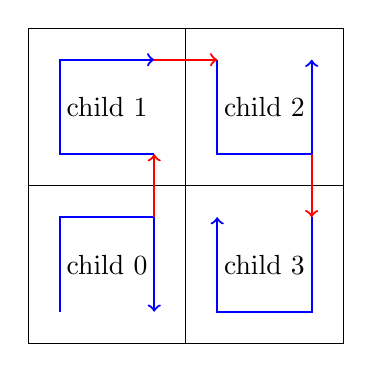
\begin{tikzpicture}[scale=2]
% Grid
\draw (0,0) rectangle (2,2);
\draw (1,0) -- (1,2);
\draw (0,1) -- (2,1);
% Labels
\node at (0.5,0.5) {child 0};
\node at (0.5,1.5) {child 1};
\node at (1.5,1.5) {child 2};
\node at (1.5,0.5) {child 3};
% Path sketch
\draw[thick,blue,->] (0.2,0.2) -- (0.2,0.8) -- (0.8,0.8) -- (0.8,0.2);
\draw[thick,blue,->] (0.8,1.2) -- (0.2,1.2) -- (0.2,1.8) -- (0.8,1.8);
\draw[thick,blue,->] (1.2,1.8) -- (1.2,1.2) -- (1.8,1.2) -- (1.8,1.8);
\draw[thick,blue,->] (1.8,0.8) -- (1.8,0.2) -- (1.2,0.2) -- (1.2,0.8);
% Connections
\draw[thick,red,->] (0.8,0.8) -- (0.8,1.2);
\draw[thick,red,->] (0.8,1.8) -- (1.2,1.8);
\draw[thick,red,->] (1.8,1.2) -- (1.8,0.8);
\end{tikzpicture}
\]
The red arrows show the gluing: exit of one child meets entry of the next.
Each gluing step crosses the face separating adjacent children.
\end{example}

%=============================================================================
\section{Levels and Active Axes}
%=============================================================================

For a hypercube with equal side lengths $2^m$ in each dimension, all $n$ axes
participate at every level of recursion. But for \emph{anisotropic} boxes
(unequal side lengths), different axes become active at different levels.

\begin{definition}[Dyadic box]
For extents $m = (m_0, \ldots, m_{n-1}) \in \NN^n$, the \emph{dyadic box} is:
\[
P(m) := \prod_{j=0}^{n-1} \{0, 1, \ldots, 2^{m_j} - 1\}.
\]
The box has $2^M$ lattice points, where $M = \sum_j m_j$.
\end{definition}

\begin{definition}[Level]
For a dyadic box with extents $m$, \emph{level $s$} refers to the $s$-th bit plane,
where $s$ ranges from 1 (finest) to $\max_j m_j$ (coarsest).
\end{definition}

\begin{definition}[Active axes]
At level $s$, the \emph{active axes} are:
\[
A_s := \{j : m_j \geq s\}.
\]
Let $k_s := |A_s|$. The active axes form a $k_s$-dimensional subcube at level $s$.
\end{definition}

\begin{proposition}
$A_{s+1} \subseteq A_s$. That is, as $s$ decreases (finer levels), axes can only activate, never deactivate.
\end{proposition}

\begin{example}[A $4 \times 2$ box]\label{ex:4x2}
For $m = (2, 1)$, we have a $4 \times 2$ box with $M = 3$ total bits.
\begin{itemize}[nosep]
\item Level 2: $A_2 = \{0\}$ (only axis 0 has $m_0 \geq 2$). This is a 1D subdivision.
\item Level 1: $A_1 = \{0, 1\}$ (both axes have $m_j \geq 1$). This is a 2D subdivision.
\end{itemize}
At level 2, we work in a 1-cube (two children). At level 1, we work in a 2-cube (four children).
Between levels 2 and 1, axis 1 ``activates.''
\end{example}

%=============================================================================
\section{Embedding}
%=============================================================================

When moving from level $s$ to level $s-1$ and new axes activate,
we must \emph{embed} the orientation from a smaller cube into a larger one.

\begin{definition}[Embedding]
Suppose $A_s \subset A_{s-1}$ (new axes activate). Given an orientation $(e, \pi)$
on the $k_s$-cube (indexed by $A_s$), we define the \emph{embedded orientation}
$(e', \pi')$ on the $k_{s-1}$-cube (indexed by $A_{s-1}$) by:
\begin{itemize}[nosep]
\item $e'_j = e_j$ for $j \in A_s$, and $e'_j = 0$ for $j \in A_{s-1} \setminus A_s$.
\item $\pi'(j) = \pi(j)$ for $j \in A_s$, and $\pi'(j) = j$ for $j \in A_{s-1} \setminus A_s$.
\end{itemize}
\end{definition}

In words: extend $e$ with 0-bits on new axes, and extend $\pi$ to fix new axes (identity on them).

\begin{lemma}[Embedding preserves adjacency]\label{lem:embed-adj}
If $u, v$ are adjacent corners in the $k_s$-cube (differing in axis $a \in A_s$),
then their embeddings $u', v'$ are adjacent corners in the $k_{s-1}$-cube (differing in the same axis $a$).
\end{lemma}

\begin{proof}
The embedding adds 0-bits on new axes, which are identical for $u'$ and $v'$.
The differing bit at axis $a$ is preserved. So $u' \oplus v' = \mathbf{e}_a$.
\end{proof}

\begin{proposition}[Embedding preserves gluing]\label{prop:embed-gluing}
If a generator satisfies the gluing condition before embedding, it satisfies it after embedding.
\end{proposition}

\begin{proof}
The gluing condition requires that $\exits(i)$ and $\entry(i+1)$ differ in axis $g(i)$.
By Lemma~\ref{lem:embed-adj}, this adjacency is preserved under embedding.
The axis $g(i)$ is in the original active set $A_s$, so it remains unchanged.
New axes have 0-bits on both sides, so they don't affect the gluing.
\end{proof}

\begin{example}[Embedding in the $4 \times 2$ box]
Continuing Example~\ref{ex:4x2}. At level 2, we have $A_2 = \{0\}$, a 1-cube.
The orientation might be $(e, \pi) = (0, \mathrm{id})$ on this 1-cube.

When axis 1 activates at level 1, we embed to $A_1 = \{0, 1\}$:
\begin{itemize}[nosep]
\item $e' = (e_0, 0) = (0, 0)$ --- the entry corner gets a 0 on the new axis.
\item $\pi'$ fixes axis 1 and acts as $\pi$ on axis 0.
\end{itemize}

The subpath that was 1-dimensional (along axis 0) now lives in a 2-dimensional space,
but the new axis 1 is ``inert'' at the level-2/level-1 boundary.
\end{example}

\begin{remark}[Why embedding is natural with $(e, \pi)$]
Contrast this with Hamilton's formulation using $(e, d)$ where $d$ is an index into
the ordered active axis list. When the list grows, $d$ must be ``reindexed'' to preserve
the physical axis. With $(e, \pi)$, we simply extend $\pi$ by the identity on new axes---there
is no reindexing. This makes the anisotropic case almost trivial.
\end{remark}

%=============================================================================
\section{The Continuity Theorem}
%=============================================================================

We can now state and prove the main result.

\begin{theorem}[Lattice continuity]\label{thm:continuity}
Let $P(m)$ be a dyadic box and $H_m: \{0, \ldots, 2^M - 1\} \to P(m)$ be the Hilbert curve
constructed using a generator satisfying the gluing condition. Then:
\[
|H_m(h+1) - H_m(h)|_1 = 1 \quad \text{for all } 0 \leq h < 2^M - 1.
\]
That is, consecutive points differ by 1 in exactly one coordinate.
\end{theorem}

\begin{proof}
The index $h$ can be written in terms of variable-width digits:
\[
h = (w_{\max}, w_{\max-1}, \ldots, w_1),
\]
where $w_s$ is a $k_s$-bit digit selecting which child at level $s$.

When $h$ increments to $h+1$, there is a smallest level $s^*$ such that:
\begin{itemize}[nosep]
\item Digits $w_1, \ldots, w_{s^*-1}$ overflow (wrap from max to 0),
\item Digit $w_{s^*}$ increments by 1,
\item Digits $w_{s^*+1}, \ldots, w_{\max}$ are unchanged.
\end{itemize}

\textbf{Case 1: Step within a child ($s^* = 1$).}
Only the finest digit changes. This is a step within a single level-1 cell,
which is a unit step by the base case.

\textbf{Case 2: Step across a child boundary ($s^* > 1$).}
The traversal moves from the last point of child $i$ to the first point of child $i+1$
at level $s^*$, where $i = w_{s^*}$ and $i+1 = w_{s^*} + 1$.

By the gluing condition (Definition~\ref{def:gluing}):
\[
\exits(i) \oplus \mathbf{e}_{g(i)} = \entry(i+1),
\]
so the exit corner of child $i$ and entry corner of child $i+1$ are adjacent along axis $g(i)$.

In lattice coordinates, the boundary between children $i$ and $i+1$ along axis $g(i)$ is:
\[
\text{coordinate } g(i): \quad 2^{s^*-1} - 1 \to 2^{s^*-1}.
\]
This is a step of exactly 1. All other coordinates are unchanged (within the same parent cell).

\textbf{Activation boundaries.}
If new axes activate between levels, Proposition~\ref{prop:embed-gluing} ensures
the gluing condition is preserved. The physical axis $g(i)$ is unchanged by embedding,
so the unit step is along the same axis before and after activation.

By induction on levels, every step in the traversal is a unit step.
\end{proof}

%=============================================================================
\section{Summary}
%=============================================================================

The key ideas:
\begin{enumerate}
\item A \textbf{Gray code} is a Hamiltonian path on the hypercube where consecutive corners are adjacent.
\item An \textbf{orientation} $(e, \pi)$ transforms a Gray code into another Gray code (Lemma~\ref{lem:orient-adj}).
\item A \textbf{generator} assigns orientations to children; the \textbf{gluing condition} ensures continuity.
\item For anisotropic boxes, \textbf{embedding} extends orientations to larger cubes by fixing new axes.
\item The \textbf{continuity theorem} follows from the gluing condition and the structure of digit overflow.
\end{enumerate}

The bit-level details (Hamilton's formulas for $e(w)$, $d(w)$, the $T$-transform)
are implementation concerns. The conceptual core is: Hilbert curves are hierarchies
of oriented Gray codes, glued along shared faces.

%=============================================================================
\appendix
\section{Hamilton's Formulas (Reference)}
%=============================================================================

For completeness, we record the explicit formulas from Hamilton's paper.

\textbf{Entry point:}
\[
e(0) = 0; \qquad e(w) = \Gray\bigl(2\lfloor(w-1)/2\rfloor\bigr) \text{ for } w > 0.
\]

\textbf{Direction (exit axis):}
\[
d(0) = 0; \qquad d(w) = \begin{cases}
\mathrm{tsb}(w-1) \mod n & \text{if } w \text{ even}, \\
\mathrm{tsb}(w) \mod n & \text{if } w \text{ odd},
\end{cases}
\]
where $\mathrm{tsb}(i)$ counts trailing set bits (trailing 1s in the binary representation).

\textbf{The $T$-transform:}
\[
T_{(e,d)}(b) = (b \oplus e) \ggg (d+1),
\]
where $\ggg$ denotes cyclic right rotation of $n$ bits.

\textbf{State update:}
\[
e' = e \oplus \rho^{-(d+1)} \cdot e(w), \qquad d' = d + d(w) + 1 \pmod{n},
\]
where $\rho$ is the cyclic permutation $\rho(a) = (a+1) \mod n$.

These formulas implement the orientation $(e, \pi)$ framework with $\pi = \rho^{-(d+1)}$,
which is why $d+1$ appears throughout. Storing $\pi$ (or equivalently $r = d+1$) directly
eliminates the offset.

\end{document}
